\section{DAPO}
\label{sec:method}

We propose the \textbf{D}ecouple Clip and \textbf{D}ynamic s\textbf{A}mpling \textbf{P}olicy \textbf{O}ptimization (DAPO) algorithm. DAPO samples a group of outputs $\{o_i\}_{i=1}^G$ for each question $q$ paired with the answer $a$, and optimizes the policy via the following objective:
\begin{equation}
\begin{aligned}
\mathcal{J}_{\text{DAPO}}(\theta) =\quad& \mathbb{E}_{(q,a)\sim \mathcal{D}, \{o_i\}_{i=1}^G\sim \pi_{\theta_\text{old}}(\cdot\mid q)}\\&
\Bigg[\frac{1}{\sum_{i=1}^{G}|o_i|}\sum_{i=1}^{G}\sum_{t=1}^{|o_i|} 
\min \Big( r_{i,t}(\theta) \hat{A}_{i,t},  
\ \text{clip} \Big( r_{i,t}(\theta), 1 - {\varepsilon_{\text{low}}}, 1 + {\varepsilon_{\text{high}}} \Big) \hat{A}_{i,t} \Big) \Bigg]
\\
\text{s.t.}\quad& 0< \Big|\{o_i\mid\texttt{is\_equivalent}(a,o_i)\}\Big|< G,
\label{eq:dapoloss}
\end{aligned}
\end{equation}
where
\begin{equation}
    r_{i,t}(\theta)=\frac{\pi_{\theta}(o_{i,t} \mid q, o_{i,<t})}{\pi_{\theta_{\text{old}}}(o_{i,t} \mid q,o_{i,<t})},\quad\hat{A}_{i,t} = \frac{R_i - \text{mean}(\{R_i\}_{i=1}^G)}{\text{std}(\{R_i\}_{i=1}^G)}.
\label{eq:advantage_calculation}
\end{equation}
The full algorithm can be found in Algorithm~\ref{algo:dapo}. In this section, we will introduce the key techniques associated with DAPO.

\subsection{Raise the Ceiling: Clip-Higher}
\label{sec:cliphigher}

In our initial experiments using naive PPO~\cite{schulman2017proximal} or GRPO~\cite{deepseekmath}, we observed the entropy collapse phenomenon: the entropy of the policy decreases quickly as training progresses (\Cref{fig:cliphigh_entropy}). The sampled responses of certain groups tend to be nearly identical. This indicates limited exploration and early deterministic policy, which can hinder the scaling process. 

We propose the \textbf{Clip-Higher} strategy to address this issue. Clipping over the importance sampling ratio is introduced in Clipped Proximal Policy Optimization (PPO-Clip)~\cite{schulman2017proximal} to restrict the trust region and enhance the stability of RL. 
We identify that the upper clip can restrict the exploration of the policy. In this case, it is much easier to make an `exploitation token' more probable, than to uplift the probability of an unlikely `exploration token'.

Concretely, when $\varepsilon = 0.2$ (the default value of most algorithms), consider two actions with probabilities $\pi_{\theta_{\text{old}}}(o_i \mid q) = 0.01$ and $0.9$. The maximum possible updated probabilities $\pi_{\theta}(o_i \mid q)$ are $0.012$ and $1.08$, respectively. 
This implies that for tokens with a higher probability (\eg, 0.9) is less constrained. Conversely, for low-probability tokens, achieving a non-trivial increase in probability is considerably more challenging.
Empirically, we also observe that the maximum probability of clipped tokens is approximately $\pi_{\theta}(o_i \mid q) < 0.2$ (\Cref{fig:max_prob_clipped}). This finding supports our analysis that the upper clipping threshold indeed restricts the probability increase of low-probability tokens, thereby potentially constraining the diversity of the system.

Adhering to the \textbf{Clip-Higher} strategy, we decouple the lower and higher clipping range as $\varepsilon_\text{low}$ and $\varepsilon_\text{high}$, as highlighted in Equation~\ref{eq:dapoloss_clip_higher}:
\begin{equation}
\begin{aligned}
\mathcal{J}_{\text{DAPO}}(\theta) = \quad&\mathbb{E}_{(q,a)\sim\mathcal{D}, \{o_i\}_{i=1}^G\sim \pi_{\theta_\text{old}}(\cdot\mid q)}\\&
\Bigg[\frac{1}{\sum_{i=1}^{G}|o_i|}\sum_{i=1}^{G}\sum_{t=1}^{|o_i|} 
\min \Big( r_{i,t}(\theta) \hat{A}_{i,t},  
\ \text{clip} \Big( r_{i,t}(\theta), 1 - {\color{red}\varepsilon_{\text{low}}}, 1 + {\color{red}\varepsilon_{\text{high}}} \Big) \hat{A}_{i,t} \Big) \Bigg]\\
\text{s.t.}\quad& 0< \Big|\{o_i\mid\texttt{is\_equivalent}(a,o_i)\}\Big|< G.
\label{eq:dapoloss_clip_higher}
\end{aligned}
\end{equation}
We increase the value of \( \varepsilon_{\text{high}} \) to leave more room for the increase of low-probability tokens. As shown in \Cref{fig:clip_high}, this adjustment effectively enhances the policy's entropy and facilitates the generation of more diverse samples.
We opt to keep \( \varepsilon_{\text{low}} \) relatively small, because increasing it will suppress the probability of these tokens to $0$, resulting in the collapse of the sampling space.

% \begin{figure}[h]
%     \centering
%     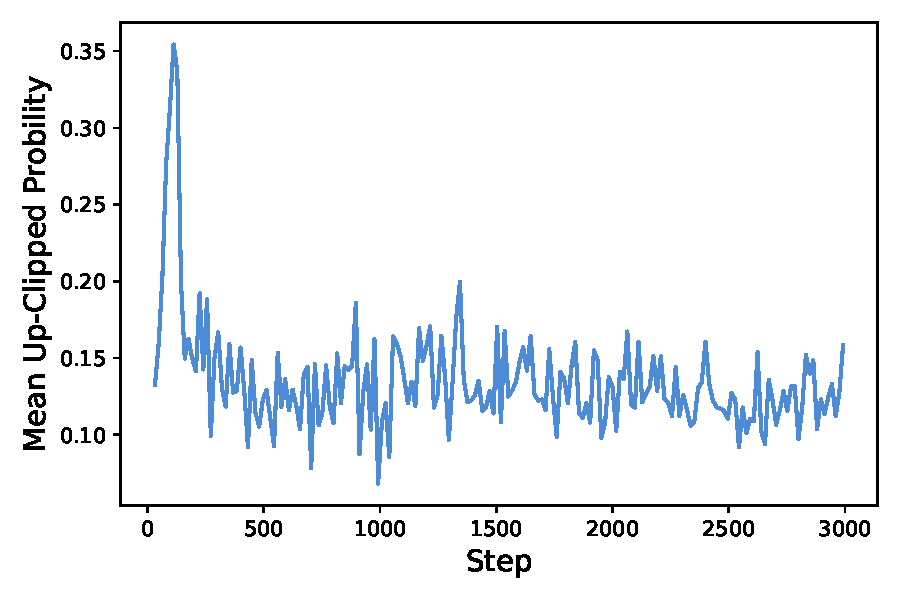
\includegraphics[width=0.5\linewidth]{figures/3.1.3.pdf}
%     \caption{Maximum clipped probabilities.}
%     \label{fig:max_prob_clipped}
% \end{figure}

% \begin{figure}[h]
%     \centering
%     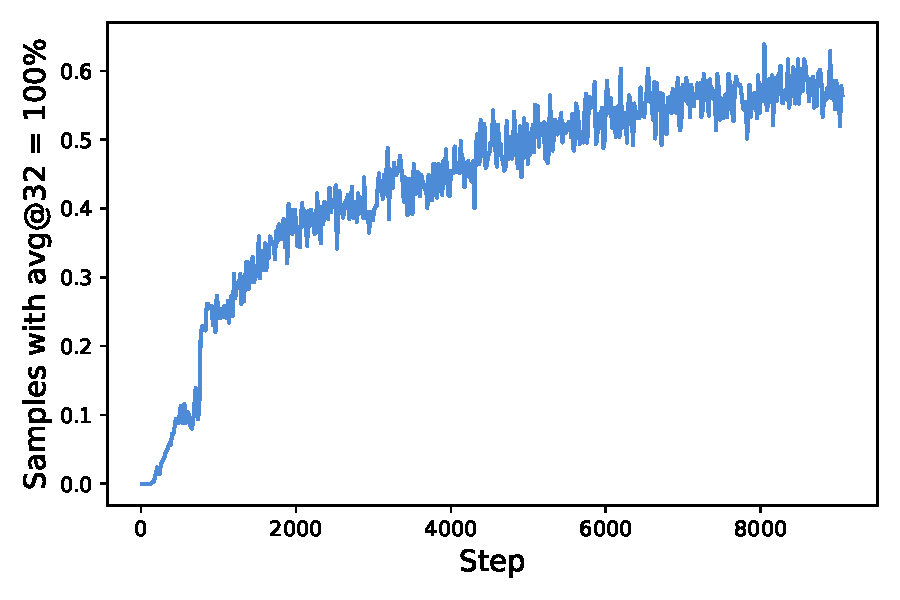
\includegraphics[width=0.5\textwidth]{figures/3.2.1.pdf}
%     \caption{The proportion of samples with an accuracy of 1 during the RL training process.}
%     \label{fig:num_samples_eq_1}
% \end{figure}

\begin{figure}
    \centering
    \begin{subfigure}{0.49\textwidth}
        \centering
        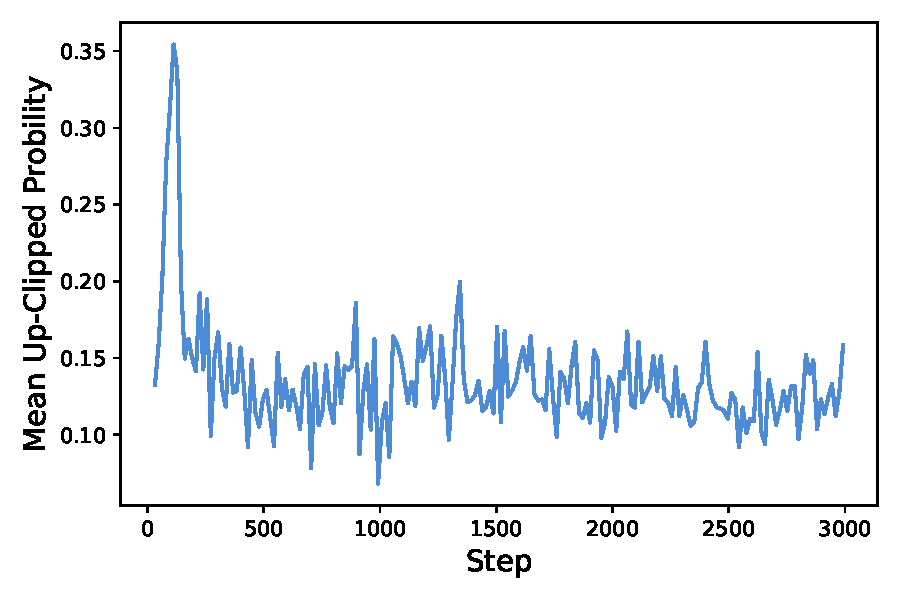
\includegraphics[width=\textwidth]{figures/3.1.3.pdf}
        \caption{Maximum clipped probabilities.}
        \label{fig:max_prob_clipped}
    \end{subfigure}
    \hfill
    \begin{subfigure}{0.49\textwidth}
        \centering
        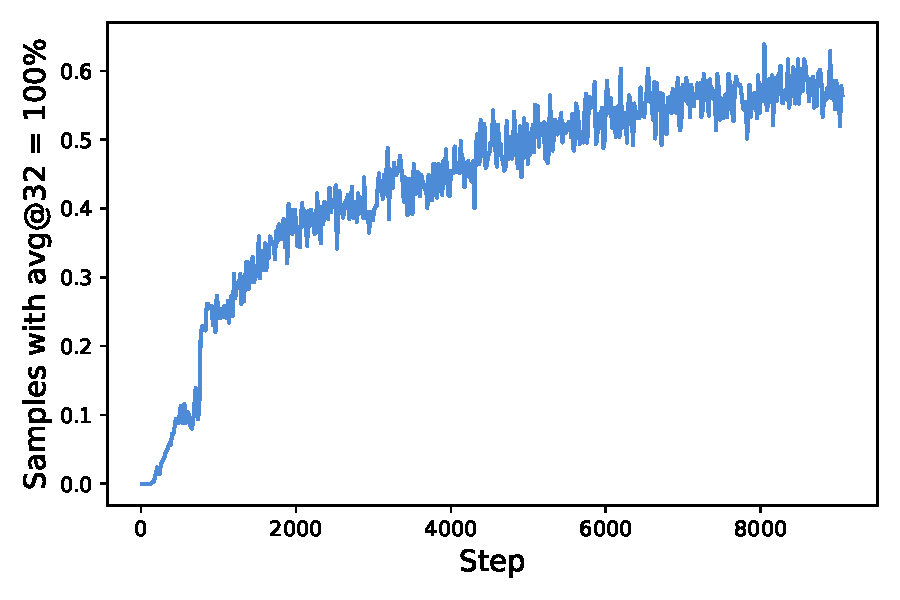
\includegraphics[width=\textwidth]{figures/3.2.1.pdf}
    \caption{The proportion of samples with an accuracy of 1.}
    \label{fig:num_samples_eq_1}
    \end{subfigure}
    
    \caption{The entropy of the probability distribution of the actor model, as well as the changes in response length.}
    \label{fig:3212}
\end{figure}

\subsection{The More the Merrier: Dynamic Sampling}
\label{sec:gradientkeeping}

Existing RL algorithm suffers from the gradient-decreasing problem when some prompts have accuracy equal to 1. For example for GRPO, if all outputs $\{o_i\}_{i=1}^G$ of a particular prompt are correct and receive the same reward 1, the resulting advantage for this group is \textit{zero}. A zero advantage results in no gradients for policy updates, thereby reducing sample efficiency. Empirically, the number of samples with accuracy equal to 1 continues to increase, as shown in \Cref{fig:num_samples_eq_1}. This means that the effective number of prompts in each batch keeps decreasing, which can lead to larger variance in gradient and dampens the gradient signals for model training.

To this end, we propose to \textbf{over-sample and filter out prompts with the accuracy equal to 1 and 0} illustrated in Equation~\ref{eq:dapoloss_oversample_filter}, leaving all prompts in the batch with effective gradients and keeping a consistent number of prompts. Before training, we keep sampling until the batch is fully filled with samples whose accuracy is neither 0 nor 1.

\begin{equation}
\begin{aligned}
\mathcal{J}_{\text{DAPO}}(\theta) =\quad& \mathbb{E}_{(q,a)\sim \mathcal{D}, \{o_i\}_{i=1}^G\sim \pi_{\theta_\text{old}}(\cdot\mid q)}\\&
\Bigg[\frac{1}{\sum_{i=1}^{G}|o_i|}\sum_{i=1}^{G}\sum_{t=1}^{|o_i|} 
\min \Big( r_{i,t}(\theta) \hat{A}_{i,t},  
\ \text{clip} \Big( r_{i,t}(\theta), 1 - {\varepsilon_{\text{low}}}, 1 + {\varepsilon_{\text{high}}} \Big) \hat{A}_{i,t} \Big) \Bigg]
\\
\text{s.t.}\quad& {\color{red}0< \Big|\{o_i\mid\texttt{is\_equivalent}(a,o_i)\}\Big|< G}.
\label{eq:dapoloss_oversample_filter}
\end{aligned}
\end{equation}

Note that this strategy does not necessarily impede training efficiency, because the generation time is typically dominated by the generation of long-tail samples if the RL system is synchronized and the generation stage is not pipelined. Besides, we find that with dynamic sampling the experiment achieves the same performance faster as shown in~\Cref{fig:afos_compare}.

% Generally, our strategy serves as a filter that screens every group of outputs and discards those rewarded with minimum or maximum scores, as these extreme samples are more likely to cluster and produce zero gradients. 
% However, a straightforward filtering approach can undermine training stability because the proportion of extreme samples varies across different batches, resulting in inconsistent numbers of useful samples at each training step. 
% To address this issue, we employ an up-sampling strategy for useful responses until the batch is fully filled. 
% Specifically, we repeat the sampling process for each prompt $q$, and subsequently discard extreme samples until the remaining samples fill the original batch size.


\subsection{Rebalancing Act: Token-Level Policy Gradient Loss}
\label{sec:tokenlevel}

The original GRPO algorithm employs a sample-level loss calculation, which involves first averaging the losses by token within each sample and then aggregating the losses across samples. In this approach, each sample is assigned an equal weight in the final loss computation. However, we find that this method of loss reduction introduces several challenges in the context of long-CoT RL scenarios.

Since all samples are assigned the same weight in the loss calculation,  tokens within longer responses (which contain more tokens) may have a disproportionately lower contribution to the overall loss, which can lead to two adverse effects.
First, for high-quality long samples, this effect can impede the model's ability to learn reasoning-relevant patterns within them.
Second, we observe that excessively long samples often exhibit low-quality patterns such as gibberish and repetitive words. Thus, sample-level loss calculation, due to its inability to effectively penalize those undesirable patterns in long samples, leads to an unhealthy increase in entropy and response length, as shown in 
\Cref{fig:token_loss_entropy} and \Cref{fig:token_loss_length}.

\begin{figure}
    \centering
    \begin{subfigure}{0.49\textwidth}
        \centering
        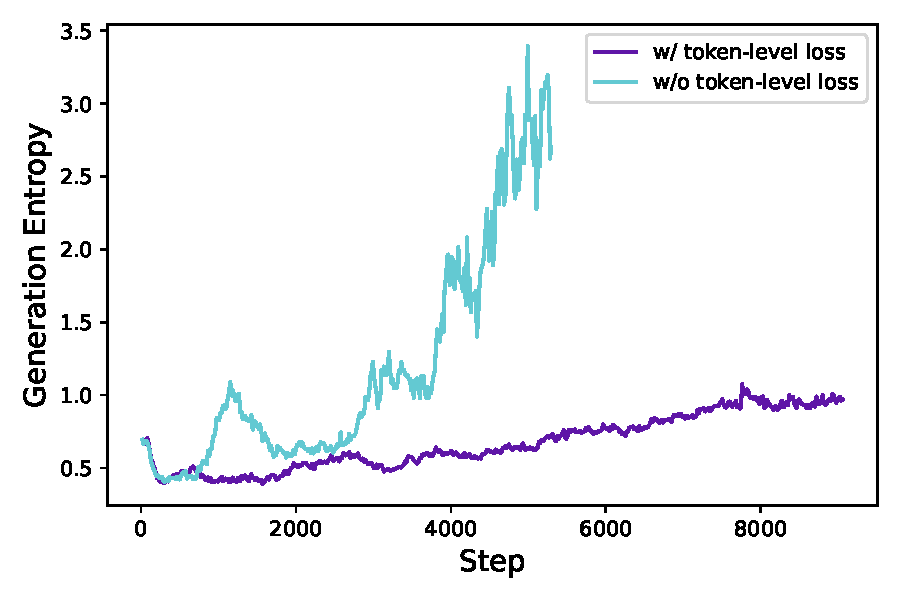
\includegraphics[width=\textwidth]{figures/3.3.1.pdf}
        \caption{Entropy of actor model's generation probabilities.}
        \label{fig:token_loss_entropy}
    \end{subfigure}
    \hfill
    \begin{subfigure}{0.49\textwidth}
        \centering
        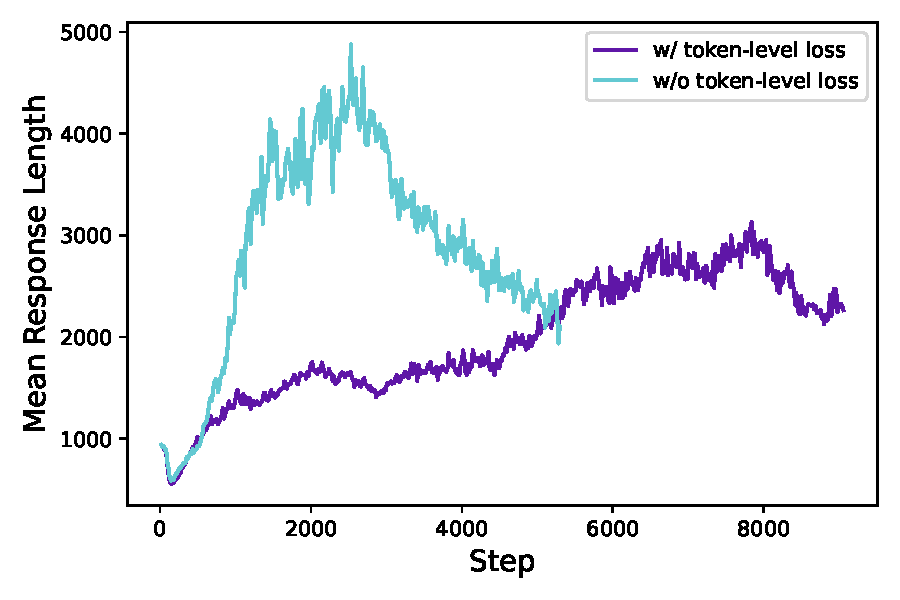
\includegraphics[width=\textwidth]{figures/3.3.2.pdf}
        \caption{Average length of actor model-generated responses}
        \label{fig:token_loss_length}
    \end{subfigure}
    
    \caption{The entropy of the probability distribution of the actor model, as well as the changes in response length.}
    \label{fig:3212}
\end{figure}

We introduce a \textbf{Token-level Policy Gradient Loss} in the long-CoT RL scenario to address the above limitations:
\begin{equation}
\begin{aligned}
\mathcal{J}_{\text{DAPO}}(\theta) = \quad&\mathbb{E}_{(q,a)\sim \mathcal{D}, \{o_i\}_{i=1}^G\sim \pi_{\theta_\text{old}}(\cdot\mid q)}\\&
\Bigg[\frac{1}{\color{red}\sum_{i=1}^{G}|o_i|}{\color{red}\sum_{i=1}^{G}\sum_{t=1}^{|o_i|}} 
\min \Big( r_{i,t}(\theta) \hat{A}_{i,t},  
\ \text{clip} \Big( r_{i,t}(\theta), 1 - {\varepsilon_{\text{low}}}, 1 + {\varepsilon_{\text{high}}} \Big) \hat{A}_{i,t} \Big) \Bigg],\\
\text{s.t.}\quad& 0< \Big|\{o_i\mid\texttt{is\_equivalent}(a,o_i)\}\Big|< G.
\label{eq:dapoloss_token_level_pg_loss}
\end{aligned}
\end{equation}
% Formally, let \( o_i \) denote a response and \( o_{i,t} \) represent the \( t \)-th token in \( o_i \), with the total number of tokens in \( o_i \) given by \( |o_i| \).
In this setting, longer sequences can have more influence on the overall gradient update compared to shorter sequences. 
Moreover, from the perspective of individual tokens, if a particular generation pattern can lead to an increase or decrease in reward, it will be equally prompted or suppressed, regardless of the length of the response in which it appears.
% The new objective function of GRPO can then be expressed as:
% \begin{equation}
% \mathcal{J}(\theta) = \mathbb{E}_{q\sim P(Q), \{o_i\}_{i=1}^G\sim \pi_{\theta_\text{old}}(O\mid q)}
% \Bigg[\frac{1}{\sum_{i=1}^{G}|o_i|}\sum_{i=1}^{G}\sum_{t=1}^{|o_i|} 
% \min \Big( r_{i,t}(\theta) \hat{A}_{i,t},  
% \ \text{clip} \Big( r_{i,t}(\theta), 1 - \varepsilon_{\text{low}}, 1 + \varepsilon_{\text{high}} \Big) \hat{A}_{i,t} \Big) \Bigg].
% \label{eq:token-level-grpo}
% \end{equation}

% \paragraph{Removal of KL Penalty} The KL penalty was originally introduced in reinforcement learning to regulate the divergence between the online policy and the frozen reference policy. In conventional RLHF settings, the goal during the RL phase is to optimize model alignment while preserving the SFT model generation patterns. However, during training of the reasoning model, the output distribution diverges significantly from base model. In this context, the KL regularization term may instead hinder training progress. Our experiments demonstrate that removing the KL penalty from the loss function leads to improved performance.

% \begin{equation}
% \mathcal{J}_{GRPO}(\theta) =
% \frac{1}{G\sum_{i=1}^{G}{|o_i|}} \sum_{i=1}^{G} \sum_{t=1}^{|o_i|} 
% \min \Bigg[
% \frac{\pi_{\theta} (o_{i,t} \mid q, o_{i,<t})}{\pi_{\theta_{old}} (o_{i,t} \mid q, o_{i,<t})} \hat{A}_{i,t}, 
% \operatorname{clip} \Bigg( 
% \frac{\pi_{\theta} (o_{i,t} \mid q, o_{i,<t})}{\pi_{\theta_{old}} (o_{i,t} \mid q, o_{i,<t})}, 1 - \varepsilon, 1 + \varepsilon 
% \Bigg) \hat{A}_{i,t}\Bigg]
% \label{eq:token-level-grpo-our}
% \end{equation}


\subsection{Hide and Seek: Overlong Reward Shaping}
\label{sec:overlong}

In RL training, we typically set a maximum length for generation, with overlong samples truncated accordingly. We find that improper reward shaping for truncated samples can introduce reward noise and significantly disrupt the training process.

By default, we assign a punitive reward to truncated samples.
This approach may introduce noise into the training process, as a sound reasoning process can be penalized solely due to its excessive length. Such penalties can potentially confuse the model regarding the validity of its reasoning process.

\vspace{5pt}
To investigate the impact of this reward noise, we first apply an \textbf{Overlong Filtering} strategy which masks the loss of truncated samples. We find that this approach significantly stabilizes training and enhances performance, as demonstrated in \Cref{fig:overlong_shaping}.

\begin{figure}[t]
    \centering
    \begin{subfigure}{0.49\textwidth}
        \centering
        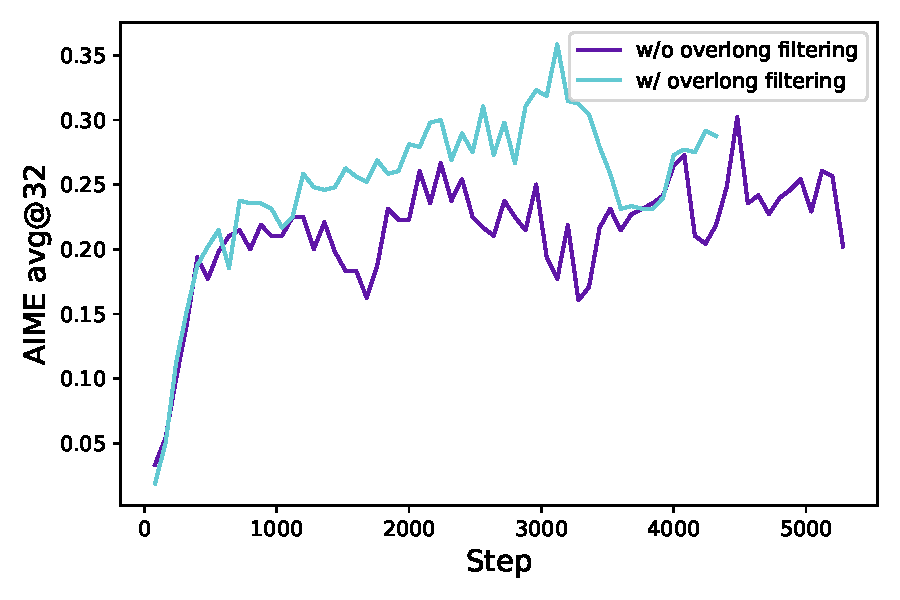
\includegraphics[width=\textwidth]{figures/3.4.1.pdf}
        \caption{Performance on AIME.}
        \label{fig:overlong_acc}
    \end{subfigure}
    \hfill
    \begin{subfigure}{0.49\textwidth}
        \centering
        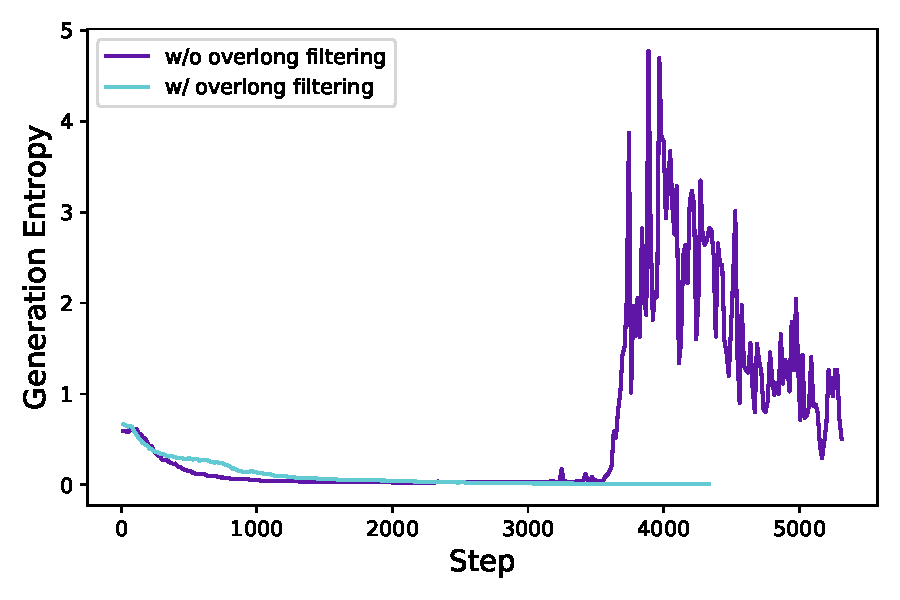
\includegraphics[width=\textwidth]{figures/3.4.2.pdf}
        \caption{Entropy of actor model.}
        \label{fig:overlong_entropy}
    \end{subfigure}
    \caption{The accuracy of the actor model on AIME and the entropy of its generation probabilities, both before and after applying \textbf{Overlong Reward Shaping} strategy.}
    \label{fig:overlong_shaping}
\end{figure}

\setcounter{table}{0}
\begin{table}[h]
    \centering
    \begin{tabular}{@{}p{1.0\textwidth}@{}} 
        \toprule 
        \textbf{Algorithm 1} \; \textbf{DAPO}: \textbf{D}ecoupled Clip and \textbf{D}ynamic s\textbf{A}mpling \textbf{P}olicy \textbf{O}ptimization \\
        \midrule 
        \textbf{Input} initial policy model $\pi_\theta$; reawrd model $R$; task prompts $\mathcal{D}$; hyperparameters $\varepsilon_\mathtt{low}, \varepsilon_\mathtt{high}$ \\
        \;1: \textbf{for} step = 1,...,M \textbf{do} \\
        \;2: \;\;\; Sample a batch $\mathcal{D}_b$ from $\mathcal{D}$ \\
        \;3: \;\;\; Update the old policy model $\pi_{\theta_{old}} \leftarrow \pi_\theta$\\
        \;4: \;\;\; Sample \textit{G} outputs $\{o_i\}_{i=1}^{G} \sim \pi_{\theta_{\text{old}}}(\cdot | q)$ for each question $q \in \mathcal{D}_b$ \\
        \;5: \;\;\; Compute rewards $\{r_i\}_{i=1}^{G}$ for each sampled output $o_i$ by running $R$ \\
        \;6: \;\;\; Filter out $o_i$ and add the remaining to the dynamic sampling buffer (\textbf{Dynamic Sampling} \Cref{eq:dapoloss_oversample_filter})\\
        \;7: \;\;\; \textbf{if} buffer size $n_b<N$: \\
        \;8: \;\;\;\;\;\;\;\; \textbf{continue} \\
            \;9: \;\;\; For each $o_i$ in the buffer, compute $\hat{A}_{i,t}$ for the \textit{t}-th token of $o_i$ (\Cref{eq:advantage_calculation}) \\
        \;10: \;\; \textbf{for} iteration = 1, ..., $\mu$ \textbf{do}\\
        \;11: \;\;\;\;\;\;\; Update the policy model $\pi_\theta$ by maximizing the DAPO objective (\Cref{eq:dapoloss})\\
        \textbf{Output} $\pi_\theta$\\
        \bottomrule
    \end{tabular}
    \captionsetup{labelformat=empty}
    \caption{}
    \label{algo:dapo}
\end{table}
\vspace{-10pt}

Furthermore, we propose \textbf{Soft Overlong Punishment} (Equation~\ref{eq:soft_punish}), a length-aware penalty mechanism designed to shape the reward for truncated samples. 
Specifically, when the response length exceeds the predefined maximum value, we define a punishment interval. Within this interval, the longer the response, the greater the punishment it receives.
%Specifically, beyond the predefined maximum length, we introduce an additional cache range for continuous soft punish where longer responses will be punished more. 
This penalty is added to the original rule-based correctness reward, thereby signaling to the model to avoid excessively long responses.


\begin{equation}
R_{\text{length}}(y) =
\begin{cases}
0, & |y| \le L_{\text{max}} - L_{\text{cache}} \\
\frac{(L_{\text{max}} - L_{\text{cache}}) - |y|}{L_{\text{cache}}}, & L_{\text{max}} - L_{\text{cache}}<|y|\le L_{\text{max}} \\
-1, & L_{\text{max}} < |y|
\end{cases}
\label{eq:soft_punish}
\end{equation}



% Therefore, we propose two improvements, \textbf{Overlong Mask} and \textbf{Overlong Punish}, to address this issue:
% \begin{itemize}
%     \item \textbf{Overlong Mask}: We exclude truncated overlong samples by masking them from group normalization calculations, which effectively reduces reward noise. 
%     However, since the model remains entirely unaware of samples that do not contribute gradient signals, it leads to an accumulation of excessively long responses in later training stages, ultimately reducing training efficiency.
%     \item \textbf{Overlong Punish}: 
% \end{itemize}

\subsection{Dataset Transformation}
\label{sec:dataprocess}

Our dataset is sourced from the AoPS\footnote{https://artofproblemsolving.com/} website and official competition homepages through a combination of web scraping and manual annotation.
The answers of math dataset typically come in a variety of formats, such as expression, formula and number, which makes it challenging to design comprehensive rules to parse them.
To provide accurate reward signals using rules and minimize errors introduced by formula parsers, inspired by AIME, we select and transform the answers into integers, which are easy to parse.
For example, if the original answer is expressed in the form of \( \frac{a + \sqrt{b}}{c} \), we instruct the LLM to modify the question so that the expected answer becomes \( a + b + c \).
After selection and transformation, we obtained the \textbf{\method-Math-17K} dataset, which consists of 17K prompts, each paired with an integer as the answer.
% Such an answer format proves to be difficult to hack.



% \newpage